\chapter{Analysis of existing methods}

  \section{Problem setup}

    \paragraph{}
    In this part we are going to set the mathematical framework for this study.
    We will start from a partial differential equation arising from the physical model, in the form of
    \begin{equation}\label{eq:pde}
      \frac{\partial \xi}{\partial t} + \operatorname{F}\left(\xi\right) = 0
    \end{equation}
    where the function $\operatorname{F}$ uses some space derivatives of the state variable $\xi$.
    This equation then describe the temporal evolution of the state variables $\xi$.

    \paragraph{}
    A particular class of such partial differential equations are conservative equations.
    They correspond to the case where the function $\operatorname{F}$ can be written as a divergence term.
    Finally, with a source term $\operatorname{S}$, those equations look like:
    \begin{equation}\label{eq:pde_conservative}
      \frac{\partial \xi}{\partial t} + \nabla \cdot \vec{\operatorname{f}}\left(\xi\right) = \operatorname{S}\ .
    \end{equation}
    One might notice that equation (\ref{eq:pde_conservative}) is indeed a particularisation of equation (\ref{eq:pde}), with $\operatorname{F}\left(\xi\right) = \nabla\cdot \vec{\operatorname{f}}\left(\xi\right) - \operatorname{S}$.
    Those conservative equations are the one we will focus on is this study, as they describe the physical systems we are interested in.

    \paragraph{}
    In this work, we will talk about computational fluid dynamics.
    We are in fact mostly interested in the Navier--Stokes equation, and its variants: the reactive Navier--Stokes equation, the Reynold-averaged Navier--Stokes equation, etc.
    A simple form of this equation can be:
    \begin{equation}\label{eq:ns}
      \left\{\begin{aligned}
        &\partial_t\left(\rho         \right) &&+ \nabla\cdot\left( \rho \vec{u} \right) &&= 0 \\
        &\partial_t\left(\rho \vec{u} \right) &&+ \nabla\cdot\left( \rho \vec{u} \otimes \vec{u} + p \id \right) &&= \nabla\cdot \mat{\tau}\\
        &\partial_t\left( \rho E      \right) &&+ \nabla\cdot\left( \left(\rho E + p\right) \vec{u} \right) &&=
          \nabla\cdot\left( \mat{\tau} \cdot \vec{u} \right)
      \end{aligned}\right.
    \end{equation}
    with the \PS{relation de fermeture} $\rho E = \frac{p}{\gamma - 1} + \rho\frac{\vec{u} \cdot \vec{u}}{2}$.
    The deviatoric stress tensor $\tau$ accounts for the viscosity of the fluid, and its computation depends on the model used.
    Without it, one recovers the Euler equations.
    To this simple form can be added source terms from the reactive model, source terms from the turbulence model, divergence terms from a diffusive model, etc.
    Yet it is clear that with a bit of rewriting, we can go back to the starting form (\ref{eq:pde}) and even the conservative form with source terms (\ref{eq:pde_conservative}).
    The quantity $\xi$ is no longer a scalar but a vector with the density $\rho$, each component of the momentum $\rho\vec{u}$ and the energy $\rho E$ as its components.
    Apart from this small change, the idea is the same.

    \paragraph{}
    When solving numerically equations like (\ref{eq:pde}), one must first take a spatial domain on interest.
    Let us call this domain $\mathcal{D}$.
    As we are interested in solving equations numerically, we need to be able to represent different quantities, such as the state variable $\xi$, numerically over the domain $\mathcal{D}$ and store it in the memory of a computer.
    Therefore we need to discretise the continuous spatial domain into a finite number of cells, or elements.
    This is usually done with a mesh of the domain $\mathcal{D}$.
    First we divide the domain $\mathcal{D}$ in a set of cells, called a mesh.
    Those cells are small volumes in 3D, faces in 2D or segments in 1D, disjoints, such as their union recovers the original domain.
    Interest quantities, such as the fluid velocity, density, \dots, are then stored at each nodes, averaged in the center of each cells or sometimes in a more complex fashion depending on the method.
    They are no longer mathematically represented by a function of the continuous physical domain $\xi : \mathcal{D} \rightarrow \mathbb{R}$ but by a finite sized vector $\Xi$ gathering all the information across the discretised domain.
    For some simple discretisation methods, this vector consists of the quantity evaluated at the mesh nodes or averaged at the center of the cells.
    For more complex methods, this vector consists of information used to construct the solution over the domain: polynomial coefficients, spectral decomposition coefficients, etc.
    Anyway, we no longer work in a continuous domain $\mathcal{D}$ but on a discretised one.

    \paragraph{}
    The partial differential equation (\ref{eq:pde}) transforms then into an ordinary differential equation:
    \begin{equation}\label{eq:ode}
      \frac{\partial \Xi}{\partial t} + \operatorname{G}\left(\Xi\right) = 0 \ .
    \end{equation}
    The difference here is that the function $\operatorname{G}$ is a function of a discrete vector whereas $\operatorname{F}$ was a function of a continuous function, and therefore $\operatorname{G}$ does not uses any spatial derivatives.
    Thanks to the spatial discretisation method, the only derivative remaining is with regard to time.
    The rest is then up to the temporal integration method, which is the main topic of this thesis.
    We will work from equation (\ref{eq:ode}) no matter where the function $\operatorname{G}$ comes from, but sometimes understanding the origin of this function can help so we will now introduce the spatial discretisation method used in our solver.


  \section{Brief introduction to the spatial integration schemes}

    \paragraph{}
    A \emph{spatial discretisation method} is the choice of how to represent a quantity over a discretised domain, and how to compute spatial derivative of this quantity from this representation.
    Indeed, before solving equation (\ref{eq:pde}) we need to decide how to transform the continuous model into a discretised one.
    We also have to look at how the spatial derivatives arising from equation (\ref{eq:pde}) translate in the discretised model.

    \subsection{The Finite Volumes method}

      \paragraph{}
      The spatial discretisation method used in the solver CHARME is called the Finite Volumes method \cite{EymardGallouetHerbin2000}.
      This method is particularly well fitted for conservatives equations such as equation (\ref{eq:pde_conservative}).
      Such equation has the property that the quantity $\xi$ is conserved: without source terms, the variation of the total quantity on $\xi$ over the domain $\mathcal{D}$ is equal to the flux $f\left(\xi\right)$ coming through the boundary $\partial\mathcal{D}$.
      In the case of the Navier--Stokes equations (\ref{eq:ns}), the density, the momentum and the energy are conserved throughout time, apart from what comes in and out of the domain.
      In a close domain where nothing comes in or out, they are indeed conserved.
      The main interest of the Finite Volumes method is that this property stays true through the spatial discretisation step.

      \paragraph{}
      The Finite Volumes method consists in integrating the partial differential equation over each cell of the mesh.
      Writing $\mathcal{V}_i$ the volume of the $i$th cell:
      \begin{equation}
        \int_{\mathcal{V}_i} \frac{\partial \xi}{\partial t} \mathrm{d}v + \int_{\mathcal{V}_i} \nabla\cdot \vec{\operatorname{f}}\left(\xi\right) \mathrm{d}v = \int_{\mathcal{V}_i} \operatorname{S} \mathrm{d}v\ .
      \end{equation}
      Then the Green--Ostrogradski theorem transforms the flux divergence into a \PS{bilan surfacique}:
      \begin{equation}
        \frac{\mathrm{d}}{\mathrm{d} t} \int_{\mathcal{V}_i} \xi\mathrm{d}v + \oint_{\partial\mathcal{V}_i} \vec{\operatorname{f}}\left(\xi\right) \cdot \vec{\mathrm{d}s} = \int_{\mathcal{V}_i} \operatorname{S} \mathrm{d}v\ .
      \end{equation}
      By writing $\square_i = \frac{1}{\norm{\mathcal{V}_i}} \int_{\mathcal{V}_i} \square \mathrm{d}v$ the average in the $i$th cell, we then have:
      \begin{equation}
        \frac{\mathrm{d}\xi_i}{\mathrm{d} t}  + \frac{1}{\norm{\mathcal{V}_i}} \oint_{\partial\mathcal{V}_i} \vec{\operatorname{f}}\left(\xi\right) \cdot \vec{\mathrm{d}s} = \operatorname{S}_i \ .
      \end{equation}

      \paragraph{}
      As stated before, the spatial discretisation method do transform the partial differential equation into an ordinary differential equation.
      It tells us to store our quantities as the averaged values represented at the center of gravity of each cells as our vector $\Xi$.
      It also tells us to compute the divergence from equation (\ref{eq:pde_conservative}) as a \PS{bilan surfacique de flux}.
      The last thing to do is to decide how to compute this \PS{bilan surfacique de flux}.
      The cells from our meshes are polygons.
      Therefore they have a finite number of (planar) faces.
      The integral over the boundary of the cell can be decomposed by the faces, to get the approximation:
      \begin{equation}
        \oint_{\partial\mathcal{V}_i} \vec{\operatorname{f}}\left(\xi\right) \cdot \vec{\mathrm{d}s} \approx \sum_{j\textrm{ neighbor of } i} \vec{\operatorname{f}}_{ij} \cdot \vec{s_{ij}}
      \end{equation}
      where $\vec{\operatorname{f}}_{ij} \cdot \vec{s_{ij}}$ is an approximation of the flux going through the face between cells $i$ and $j$.
      This approximation is a key element of the Finite Volumes method, therefore we will discuss it later.
      We can now compute the function $\operatorname{G}$ from equation (\ref{eq:ode}): for each face of the mesh we compute $\vec{\operatorname{f}}_{ij} \cdot \vec{s_{ij}}$, we add this value to the $i$th component and remove it from the $j$th component of our new vector.
      Then, after adding the source terms we get a vector containing the result of $\operatorname{G}\left(\Xi\right)$.
      As can be seen, every contribution of the flux added in a cell is removed from another, and therefore this spatial discretisation method preserves the conservativity of the underlying equation.


    \subsection{The Riemann problem}

      \PS{Déplacer après la reconstruction ? C'est plus fondamental mais ça intervient après}

      \paragraph{}
      The last remaining problem with this presentation of the Finite Volumes method is how to compute the flux going through cell interfaces.
      On the interfaces between two cells we know the left and right quantities $\xi_L$ and $\xi_R$, and we need to compute the corresponging flux.
      It is possible here to use a reconstruction method to get a better approximation of the quantities left and right of the interface, and therefore we end up using the left and right quantities $\xi_L^*$ and $\xi_R^*$.
      The idea is now to compute the flux going through the face as a function of $\xi_L^*$, $\xi_R^*$ and the surface vector $\vec{s}$.
      From the interface point of view, there are two possibly different states, one from each side: this is what is called a Rienamm problem.
      A Riemann problem is an initial value problem applied to a conservation equation, where the initial solution is piecewise constant with a single possible discontinuity.
      By working with the equation and deriving the jump condition, it is possible to compute the quantity at the interface from a possibly discontinuous state at the interface.
      Then it is possible to evaluate the flux associated with this state going through the surface.
      This approach can be called the exact Riemann solver as it uses the exact solution of the Riemann problem.
      But the drawback from this approach usually is the computational coast required to find this exact solution.
      What is usually done is to use approximate Riemann solvers, compromising between speed and accuracy.
      Several Riemann solvers\footnote{\PS{Est-ce qu'on parle toujours de solveur de Riemann (qui trouve la solution du problème idoine) ou on parle de "schéma de flux numérique" ?}} are available to the user in our solver, such as the well known Roe, HLLC or AUSM+ schemes \cite{Roe1981, Toro2009}.


    \subsection{Gradient reconstruction methods}

      \paragraph{}
      The standard Finite Volumes method represent quantities with the averaged value in each cell.
      This correspond to a first order discretisation method.
      Simply put, it means that it can represent quantities exactly as 0 order polynomials locally to each cell.
      There are ways to achieve a higher order representation such as with the MUSCL approach \PS{(ref nécessaire ?)}.
      It consists in handling the surface flux evaluation on one hand, which is what we did in the Riemann problem part, and deciding what left and right quantities to feed to this flux computation on the other hand.
      In our solver, there are two ways to construct high order states to give to the flux computation method.
      They are described in the following parts.
      For both of them, the idea is to use neighboring data to enhance the order of the local representation.


      \subsubsection{The $k$-exact method}

        \paragraph{}
        The first method used to reconstruct high order quantities is called the \emph{$k$-exact} method.
        The idea is to construct iteratively an order $k$ representation of the quantity using the neighboring order $k-1$ representation \cite{HaiderCroisilleCourbet2009}.
        Usually, as do most of the solver users, this method is used to achieve a second order reconstruction.
        But it can also achieve higher order reconstructions \cite{HaiderCroisilleCourbet2011, HaiderCourbetCroisille2018, PontBrennerCinellaEtAl2017}.
        At each step, while increasing the order of the representation, it is important not to create a local maximum or minimum.
        This might happen close to discontinuities in the solution, or near rapidly varying spots \PS{reformuler}.
        It is indeed common, when interpolating, to create local overshoot or undershoot.
        One might think here about the Gibbs or Runge's phenomena, and despite here being a different problem the idea is the same.
        Creating local extrema in the solution can be troublesome, and so the $k$-exact method limits the reconstructed polynomial to ensure it does not.


      \subsubsection{The Multislope method}

        \paragraph{}
        The second method used to reconstruct high order quantities is called the \emph{Multislope} method.
        At each face, this method computes a local gradient to interpolate the quantity from the center of the cell to the face.
        This gradient is obtained using neighboring data, with a complex mechanism that we will not discuss here \cite{LeTouzeMurroneGuillard2015}.
        Finally, the Multislope method gives a second order reconstruction.
        Once again, this reconstruction might create local maxima or minima, and therefore it uses slope limiters \cite{Venkatakrishnan1993, BergerAftosmis2005} to prevent it.


      \paragraph{}
      We briefly explained above the spatial discretisation method used in our solver, as it might help our analysis on the time integration part.
      The Finite Volumes method averages the partial differential equation over each cell of the mesh, which transforms the flux divergence into a \PS{bilan surfacique de flux}.
      A reconstruction method, the $k$-exact method or the Multislope method, is then used to get a higher order representation of the solution so that the surface flux can be computed at each face.
      Slope limiters are used to prevent the formation of local extrema, which can be harmful to the computation.


  \section{Time integration methods}

    \paragraph{}
    With the help of a spatial discretisation method, the equation we want to solve is now an ordinary differential equation.
    The main objective of this thesis is focused on the resolution of steady problems.
    The steady solution of equation (\ref{eq:ode}) is given by $\operatorname{G}\left(\Xi\right) = 0$.
    To get the solution, one might then try to find a root of the function $\operatorname{G}$.
    Unfortunately, with our typical applications, this function $\operatorname{G}$ has got bad mathematical properties, such as its stiffness, arising from the nonlinearities of the underlying equations.
    Therefore, algorithms that try to find a root of $\operatorname{G}$ struggle and usually fail.
    Another approach is to take an initial value $\Xi_0$, and to solve the equation (\ref{eq:ode}) for this initial value.
    After a long enough time, we hope that $\Xi$ will reach the desired steady solution.

    \paragraph{}
    The idea is now to solve the temporal evolution of $\Xi$ to get the solution after a long time, when it approaches the steady solution.
    We will solve the equation numerically, which mean we will iteratively compute the next solution after a given time step, knowing the current one.
    Is is also possible to modify the equation, as we are interested in the final state, not in the transient one.
    It is possible for example to use local time stepping, which consists in having each cell of the mesh moving forward in time with its own time step.
    The resulting transient states do not make sense from a physical point of vue, as the equation solved is not the initial one, but it converges to the same steady solution.
    Therefore, it is alright to change the equation as long as it gives the same steady solution.
    Finally, this way of finding a converged steady solution is what is called a \emph{Pseudo-Transient Continuation} method \cite{KelleyKeyes1996}.

    \paragraph{}
    After deciding on an initial value, the equation we now want to solve is:
    \begin{equation}\label{eq:init_value_ode}
      \left\{\begin{aligned}
        & \frac{\mathrm{d} \Xi}{\mathrm{d}t} + \operatorname{G}\left(\Xi\left(t\right)\right) = 0 \\
        & \Xi\left(t_0\right) = \Xi_0
      \end{aligned}\right. \ .
    \end{equation}
    A time integration method is going to produce a succession of solutions: starting from $\Xi_0$, it produces $\Xi_1$ at $t_1$, then $\Xi_2$ at $t_2$, and $\Xi_n$ at $t_n$, etc.
    We will note $\Delta t_n$ the time step $t_{n+1} - t_n$.
    As we will mostly look at single steps of the time integration methods in the following, we will drop the subscript on the time step when it is not meaningful.
    We want to find the steady solution, and we are not interested in the evolution of the solution.
    It seems then reasonable to want to "go fast" to the steady state, meaning to use as large a time step as possible.
    Unfortunately, not every time integration method allows large time steps, as is well known \cite{CourantFriedrichsLewy1967}.
    We need to define some tool to help us decide on the method we will use.


    \subsection{Analysis of time integration methods}

      \subsubsection{Consistency and order}

        \paragraph{}
        A time integration method must respect some properties to be "well behaved".
        For instance, it have to be consistent.
        To define the consistency, we look at equation (\ref{eq:init_value_ode}).
        After one step, a numerical method gives a value $\Xi_1$, believed to be near the exact value $\Xi\left(t_0 + \Delta t\right)$.
        A numerical time integration method is said to be consistent if:
        \begin{equation}
          \lim_{\Delta t \rightarrow 0} \frac{\Xi_1 - \Xi\left(t_0 + \Delta t\right)}{\Delta t} = 0 \ .
        \end{equation}
        Also, the method is of order $p$ if the local error is in $\Delta t^{p+1}$ \cite{Iserles2008}:
        \begin{equation}
          \Xi_1 - \Xi\left(t_0 + \Delta t\right) = O\left(\Delta t^{p+1}\right) \ .
        \end{equation}
        This means a $p$ order method can recover exactly a solution that is a polynomial function of time of order less or equal to $p$.

        \paragraph{Note:}
        % The order of a spatial discretisation method reflect its "local" behavior,
        The order of a time integration method reflect its "local" behavior, meaning on a single given time step, provided it is small enough.
        In the field of spatial discretisation of partial differential equations, the order $p$ of a method is such as:
        \begin{equation}
          \norm{\Xi - \Xi_{exact}} = O\left(h^p\right)
        \end{equation}
        where $h$ is the spatial discretisation parameter.
        We notice a difference between the two definitions: the error order of magnitude is $p+1$ for the temporal method and $p$ for the spatial one.
        This is due to the fact that the error we look at in the spatial case is global: it sums the error over the whole domain.
        It would correspond to counting the error on each step for the temporal integration.
        To convince oneself, we could say that when solving the differential equation \PS{on/in} an interval $\left[0, T\right]$ with a fixed $T$, the global error of a $p$ order method would \PS{be of, in, behave like ?} $O\left(\Delta t^p\right)$ as it amount to summing $T/\Delta t$ local errors of $O\left(\Delta t^{p+1}\right)$.
        We then get the coherency with the definition of the order for spatial discretisation methods.
        If this trick can help understand the difference between the two definitions, this is indeed just a mental trick and not a sound mathematical proof.
        To get this proof, more hypothesis on the method are required \cite{Iserles2008}.


      \subsubsection{Stability}

        \paragraph{}
        A meaningful criteria in the choice of a time integration method is the stability.
        Depending on the application, we will expect different level of stability in order to avoid a numerically induced divergence of the computation.

        \paragraph{}
        To analyse the stability of a time integration method, we usually apply it on the ordinary differential equation with a lineal right hand side: the Dahlquist test equation \cite{HairerWanner1996}.
        The reason is that if we have a solution $\tilde{\Xi}$ of equation (\ref{eq:init_value_ode}), we can linearise $\operatorname{G}$ in $\tilde{\Xi}$.
        With $y = \Xi - \tilde{\Xi}$ and $J = -\frac{\partial \operatorname{G}}{\partial \Xi}\left(\tilde{\Xi}\right)$, assumed constant, we then have:
        \begin{equation}\label{eq:dahlquist}
          \frac{\mathrm{d} y}{\mathrm{d} t} = J y \ .
        \end{equation}
        This new equation used to analyse the stability of time integration methods is the one called the Dahlquist test equation.
        We look at this equation in $\mathbb{C}$, so that we can compute the eigenvalues and eigenvectors of the matrix $J$.

        \paragraph{Note:}
        When looking at a method applied to the Dahlquist test equation (\ref{eq:dahlquist}), we assume that the real part of the eigenvalues of $J$ are all negative.
        This choice may seem arbitrary but can be understood with the following example.
        Let us work in $\mathbb{C}^2$, with:
        \begin{equation}
          J = \begin{pmatrix} -1 & 0 \\ 0 & 10^3 \end{pmatrix}, \quad y_0 = \begin{pmatrix} 1 \\ 0 \end{pmatrix} \ .
        \end{equation}
        The solution of the equation is then :
        \begin{equation}
          y\left(t\right) = \begin{pmatrix} e^{-t} \\ 0 \end{pmatrix} \ .
        \end{equation}
        As we solve the equation numerically, the floating point representation introduce some roundoff error.
        The initial condition may then be
        \begin{equation}
          y_0' = \begin{pmatrix} 1 \\ \epsilon \end{pmatrix}
        \end{equation}
        instead of the exact one $y_0$, with a typical $\epsilon = 10^{-15}$ for double precision.
        Let us suppose that we have an exact time integration method that gives the exact solution at each time step $t_n = n\Delta t$.
        The solution computed by this method will be:
        \begin{equation}
          y_n = \begin{pmatrix} e^{-n\Delta t} \\ \epsilon e^{10^3 n \Delta t} \end{pmatrix}
        \end{equation}
        that gives an error of $\epsilon e^{10^3 n\Delta t}$.
        For the numerical values suggested here, this amount to an error as large as $10^6$ for $n = 5$ and $10^{28}$ for $n = 10$.
        The explosion of the error comes from the fact that the positive eigenvalue of $J$ amplifies the roundoff error.
        This phenomenon has nothing to do with the time integration scheme, but with the equation.
        Finally, this is why we study equation (\ref{eq:dahlquist}) assuming the eigenvalues of $J$ are negative.


        \paragraph{Single step methods}
        To compute the solution at the next time step, some method need only to know the current solution.
        Such methods are called single steps methods.
        When applied to the Dahlquist test equation (\ref{eq:dahlquist}), we write for a single step method:
        \begin{equation}\label{eq:single_step}
          y_{n+1} = g\left(\Delta tJ\right)y_n
        \end{equation}
        the relationship between the current solution and the next one.
        For most time integration methods, $g$ is an analytic function.
        By decomposing the initial value on a basis of eignevectors of $J$, $v_1, \dots, v_N$, associated to the eigenvalues $\alpha_1, \dots, \alpha_N$, we write: $y_0 = \sum_{i=1}^N \lambda_i v_i$.
        Because $g$ is an analytic function, we then have:
        \begin{equation}
          y_n = \sum_{i=1}^N \lambda_i g\left(\Delta t \alpha_i\right)^n v_i \ .
        \end{equation}

        It is now straightforward to deduce a stability condition for the single step method: if for any $i$ we have $\left|g\left(\Delta t\alpha_i\right)\right| < 1$, then $y_n$ converges to 0.
        This is how we can define the stability region of a time integration method:
        \begin{equation}
          \left\{ \, z \in \mathbb{C} \; \mid \; \left| g\left(z\right) \right| < 1 \, \right\} \ .
        \end{equation}
        When each eigenvalue of $J$ falls in the stability region, then the method is stable.

        \paragraph{}
        If an eigenvalue is not in the stability region, the associated \PS{direction propre} will be amplified and a numerical instability will lead to the divergence of the computation.
        We can see that the argument of the function $g$ is not $J$ but $\Delta t J$.
        This means that the stability can be achieved by choosing wisely the time step: with a small enough $\Delta t$ we can make sure that each eigenvalue falls into the stability region.
        Unfortunately, this often force the user to set a relatively small time step, which is an issue for our steady computations.


        \paragraph{Multi step methods}
        Some methods do not fall in the previous framework.
        The multi step methods, in particular, cannot be written under the form of equation (\ref{eq:single_step}).
        These methods use not only $y_n$ to find $y_{n+1}$, but the $k$ previous steps.
        Applied to equation (\ref{eq:dahlquist}), they can be written in the form:
        \begin{equation}
          y_{n+1} = \sum_{i=1}^k g_{k-i}\left(\Delta t J\right) y_{n+1-i} \ .
        \end{equation}
        When we look for $y_i$ under the form $y_i \propto \mu^{i}$, we then have:
        \begin{equation}
          \mu^k = \sum_{i=1}^k g_{k-i}\left(\Delta t J\right) \mu^{k-i}
        \end{equation}
        which leads us to identifying the polynomial $g_{\Delta t J}\left(\mu\right) = \mu^k - \sum_{i=0}^{k-1}g_i\left(\Delta t J\right)\mu^i$.
        If each root of this polynomial is of modulus less than 1, the solution converge to 0.
        This is how we can define the stability region for multi step methods \cite{HairerWanner1996}:
        \begin{equation}
          \left\{ \, z \in \mathbb{C} \; \mid \; \parbox{25em}{all roots of $X^k - \sum_{i=0}^{k-1}g_i\left(z\right)X^i$ are of modulus less or equal to 1, strictly less to 1 for roots with multiplicity}
           \, \right \} \ .
        \end{equation}

        \paragraph{}
        The key property resulting in the stability analysis of time integration methods is the \emph{A-stability} \cite{Dahlquist1963}.
        A time integration method is A-stable if its stability region contains the left half complex plane.
        Simply put, a method is A-stable if it converges to 0 when it should, and does not diverge due to numerical errors.
        The A-stability is interesting to us, as an A-stable method is also said to be unconditionally stable, whereas a method that is not is conditionally stable.
        This other characterisation comes from the fact that a non A-stable method needs to respect some additional criteria to be stable, on the time step it uses for example, whereas an A-stable method is stable no matter the time step.
        As we said before, we would like to use large time steps to quickly get the steady state on our applications, and that is why  we look for A-stability in out methods.

    \subsection{Explicit methods}

      \paragraph{}
      Explicit methods are called this way because at each step, the computation of the next solution is straightforward: they give it explicitly as a function of current available data.
      They are largely used in unsteady computational fluid dynamic simulations.
      Their strength comes from the fact that they are usually simple and therefore easy to implement in a solver, and computationally inexpensive compared to non explicit methods.


      \subsubsection{Explicit Euler method}

        \paragraph{}
        The explicit Euler method is the most simple time integration method.
        It consists in integrating equation (\ref{eq:init_value_ode}) between $t_n$ and $t_{n+1}$ assuming the function $\operatorname{G}$ stays constant, equal to $\operatorname{G}\left(\Xi_n\right)$.
        Equivalently, it consists in replacing the time derivative $\frac{\mathrm{d} \Xi}{\mathrm{d} t}$ by a finite difference $\frac{\Xi_{n+1} - \Xi_n}{\Delta t}$.
        Then, the method gives:
        \begin{equation}
          \Xi_{n+1} = \Xi_n - \Delta t \operatorname{G}\left(\Xi_n\right) \ .
        \end{equation}

        \paragraph{}
        After verifying that this is a first order method, a quick stability analysis gives a stability region equal to the open unity disk centered in -1.
        Practically, this stability region is often deemed unsatisfactory as it forces the use of small time steps.
        Yet this method is a classic that we had to introduce before talking about more complex methods.


      \subsection{Runge--Kutta methods}

        \paragraph{}
        Instead of making one step forward in time as the explicit Euler method, the Runge--Kutta methods will make a set of intermediate steps, and the final solution is found as a combinaison of those intermediate steps.
        The general idea is as such.
        Supposing we know the value of $\Xi_n$ in $t_n$, we set the intermediates steps $t_{n, i} = t_n + c_i\Delta t$ for $1 \leq i \leq k$, with a fixed $k$.
        We can now integrate exactly between $t_n$ and $t_{n, i}$ equation (\ref{eq:init_value_ode}):
        \begin{equation}
          \Xi\left(t_{n, i}\right) = \Xi_n - \Delta t \int_{t_n}^{t_{n,i}} \operatorname{G}\left(\Xi\left(t\right)\right) \mathrm{d}t\ .\
        \end{equation}
        The integral on the right hand side is then approximated with a \PS{quadrature} using the previously computed intermediate steps:
        \begin{equation}
          \int_{t_n}^{t{n,i}} \operatorname{G}\left(\Xi\left(t\right)\right) \mathrm{d}t \approx \sum_{j = 1}^{i-1} a_{ij} \operatorname{G}\left(\Xi\left(t_{n,j}\right)\right) \ .
        \end{equation}
        Once each intermediate step in known, we finally integrate between $t_n$ and $t_{n+1}$ equation (\ref{eq:init_value_ode}) and approximate the integral using the intermediate steps.

        \paragraph{}
        To sum up, a Runge--Kutta method iterates in the following way:
        \begin{equation}
          \left\{\begin{aligned}
            \Xi_{n+1} &= \Xi_n - \Delta t \sum_{i = 1}^k b_i \operatorname{G}\left(\Xi_{n,i}\right) \\
            \textrm{with}\quad \Xi_{n,i} &= \Xi_n - \Delta t \sum_{j = 1}^{i-1} a_{ij} \operatorname{G}\left(\Xi_{n,j}\right)
          \end{aligned}\right. \ .
        \end{equation}

        \paragraph{}
        A Runge--Kutta method is characterised by its size $k$ and the quadrature coefficients $a_{ij, 1\leq j<i\leq k}$, $b_{i, 1\leq i\leq k}$ and $c_{i, 1\leq i\leq k}$.
        There are as many Runge--Kutta methods as there are choices in the quadrature coefficients, but not all choices give good methods.
        There are criteria that the coefficients must follow to ensure the consistency of the method, and then criteria with more complexity as the order increases.
        The quadrature coefficients are often arranged in the Butcher tableau:
        \begin{equation}
          \begin{array}{c|c}
            c & A \rule[-1.1ex]{0pt}{0pt} \RKBar b^T
          \end{array}
          \qquad = \qquad
          \begin{array}{c|ccccc}
            0\\
            c_2    & a_{21} \\
            c_3    & a_{31} & a_{32} \\
            \vdots & \vdots &        & \ddots\\
            c_k    & a_{k1} & a_{k2} & \hdots & a_{k,k-1} \RKBar
            b_1    & b_2    & \hdots & b_{k-1} & b_k
          \end{array} \ .
        \end{equation}

        \begin{table}
          \begin{tabular}{P{.15\textwidth}P{.3\textwidth}P{.4\textwidth}}
            \begin{tabular}{c|c}
              0 \RKBar 1
            \end{tabular} &
            \begin{tabular}{c|cc}
              0 \\ 1/2 & 1/2 \RKBar 0 & 1
            \end{tabular} &
            \begin{tabular}{c|cccc}
              0 \\ 1/2 & 1/2 \\ 1/2 & 0 & 1/2 \\ 1 & 0 & 0 & 1 \RKBar 1/6 & 1/3 & 1/3 & 1/6
            \end{tabular} \\
            RK1 & RK2 & RK4 \\
          \end{tabular}
          \caption{Butcher tableau for the explicit Euler, Midpoint and RK4 methods}\label{tab:rk_butcher}
        \end{table}

        \paragraph{}
        The Butcher tableau of some well known Runge--Kutta methods are shown in table \ref{tab:rk_butcher}.
        The RK1 method is in fact equivalent to the explicit Euler method.
        The RK2 method is one of the 2 steps second order Runge--Kutta method.
        This one is also called the Midpoint method.
        The RK4 method is a fourth order method with 4 steps.
        This is the most famous Runge--Kutta method, vastly used for explicit time integration of ordinary differential equations.

        \paragraph{}
        It can be shown that the order $p$ of the method less or equal to the number of steps $k$.
        Up to 4 steps, it is possible to chose the quadrature coefficients to have $p = k$.
        Above that, getting a bound on the order depending on the number of steps is still an open problem as of today.
        For a Runge--Kutta method of order $p$, the corresponding function used for the stability analysis is \cite{HairerWanner1996}:
        \begin{equation}
          g\left(z\right) = 1 + z + \frac{z^2}{2} + \dots + \frac{z^p}{p!} + O\left(z^{p+1}\right) \ .
        \end{equation}
        When $p = k$, the last term $O\left(z^{p+1}\right)$ is in fact null.
        We show on the figure \ref{fig:rk_stab} the stability region of the Runge--Kutta methods of orders up to 4.

        \begin{figure}
          \centering
          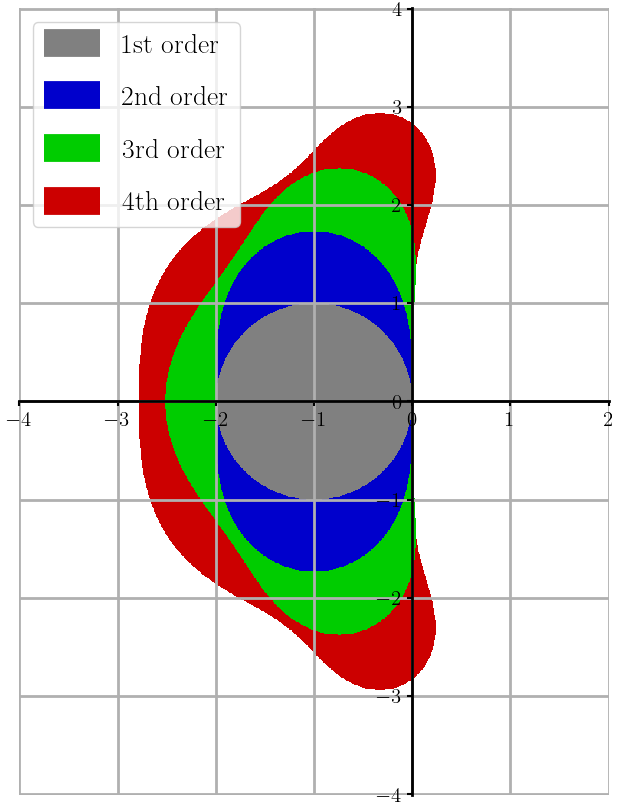
\includegraphics[width=.45\textwidth]{figures/rk_stab.png}
          \caption{Stability regions (in color) of the four first order Runge--Kutta methods.}
          \label{fig:rk_stab}
        \end{figure}

        \paragraph{}
        We can see that Runge--Kutta methods are not A-stable, and they do not have a large stability region.
        Increasing the order of the method does increase the stability region, but not enough for our applications.
        Practically, this impose the use of small time steps, which is agreeable for unsteady computations but not for our steady ones.
        If ont iteration of the method is inexpensive, the total number of iterations needed to reach the steady solution will make the overall computation too costly.


      \subsection{Adams--Bashforth methods}

        \paragraph{}
        We could try to use other explicit methods, such as the multi step Adams--Bashforth methods.
        The $k$th order Adams--Bashforth method uses the last $k$ computed steps to find the next one.
        One can indeed check that the index $k$ designating the method also corresponds to its order \cite{HairerNorsettWanner1993}.

        \paragraph{}
        The idea is to apply a Lagrange interpolation of the function $\operatorname{G}$ from equation (\ref{eq:init_value_ode}) in the $k$ last computed points, and then replace $\operatorname{G}$ with the interpolation polynomial when integrating from $t_n$ to $t_{n+1}$.
        Contrary to the Runge--Kuta methods, as we reuse previous information, a single $\operatorname{G}$ evaluation is required at each step.
        The coast of one iteration of the Adams--Bashforth method is then really cheap \PS{(reformuler)}.
        The stability analysis for such methods is a bit more complex \cite{HairerNorsettWanner1993, HairerWanner1996}, and so we show the result that we obtained numerically on figure \ref{fig:ab_stab} without \PS{faire le calcul : deriving the calculus ?}.
        The conclusion is even worse than with the Runge--Kutta methods, as the stability region decreases as the order increases.
        The Adams--Bashforth can reach a high order of accuracy while staying computationally inexpensive, but they lack drastically of stability, and that is why they are often not used in computational fluid dynamics computations.
        More generally, an explicit multi step method cannot be A-stable \cite{Dahlquist1963}.

        \begin{figure}
          \centering
          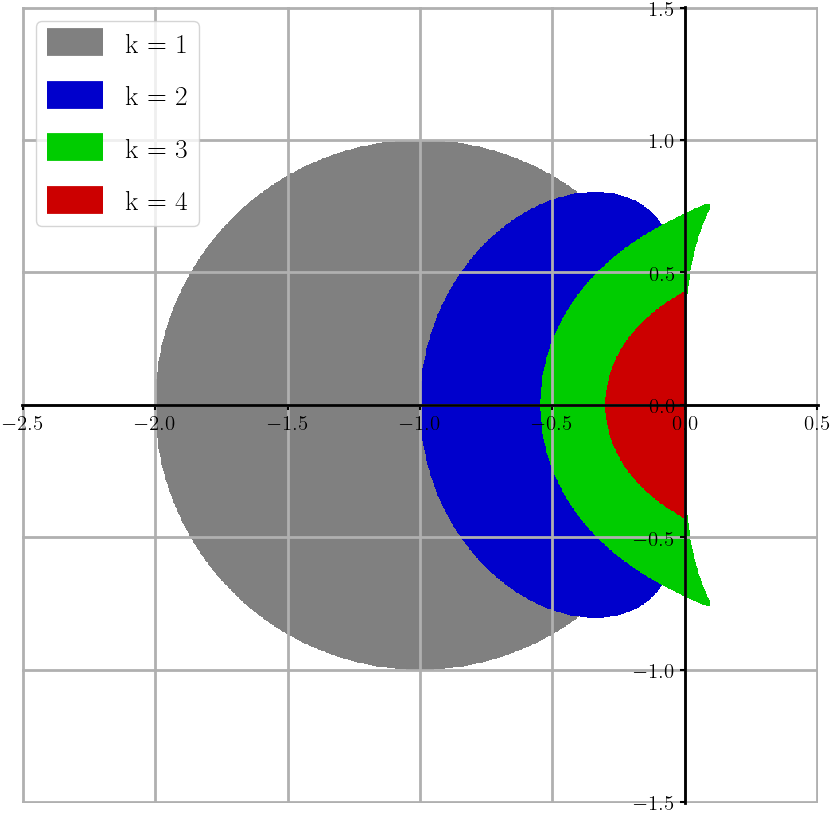
\includegraphics[width=.6\textwidth]{figures/ab_stab.png}
          \caption{Stability regions (in color) of the four first Adams-Bashforth methods.}
          \label{fig:ab_stab}
        \end{figure}


    \subsection{Méthodes implicites}

      \subsubsection{Méthode d'Euler implicite}


      \subsubsection{Principe des méthodes implicites}
